\documentclass[11pt, a4paper]{article}
%\usepackage{proj1}
\usepackage{natbib}
\usepackage{fancyhdr}  
\usepackage{subcaption}
\usepackage{caption}
\usepackage{graphicx}
\linespread{1.25} 
\setlength{\parindent}{0cm}
\graphicspath{{Images/}}
\usepackage{hyperref}
\usepackage{amsmath}
\usepackage{amsfonts}
\usepackage{amssymb}
\usepackage{amsthm}
\usepackage{mathtools}
\usepackage{commath}

%\usepackage[sc,osf]{mathpazo}
\usepackage{subcaption}
\usepackage[a4paper, top=1in, left=1.0in, right=1.0in, bottom=1in, includehead, includefoot]{geometry} %Usually have top as 1in

\usepackage{listings}
\usepackage{color} %red, green, blue, yellow, cyan, magenta, black, white
\definecolor{mygreen}{RGB}{28,172,0} % color values Red, Green, Blue
\definecolor{mylilas}{RGB}{170,55,241}


\hypersetup{colorlinks,linkcolor={black},citecolor={blue},urlcolor={black}}
\usepackage{color}
\urlstyle{same}


\theoremstyle{definition}
\newtheorem{definition}{Definition}[section]

\title{Exact Solutions for the Full Problem \\with Force Control and with Flow Control}
\date{}
\newcommand{\Sta}{\rho}
\newcommand{\Adj}{p}
\newcommand{\Con}{u}

\pagenumbering{gobble}
\begin{document}
	
\section*{Report 30/04/2020}
All plotting times are defined by 'linspace(0,1,10)'. All examples are run with FixPt, and $\beta = 10^{-3}$ only. $\lambda = 0.01$, $N= 60$, $n = 61$, OLD Tol $= 10^{-8}$, Optimality Tol $=10^{-4}$.

\section{Neumann Flow Control - Asymmetric Example 1}
For this, the initial condition for $\rho$ is $\rho_{IC}=0.5$, and the Flow term is zero in the forward problem.
The target is:
\begin{align*}
\hat \rho = 0.5(1-t) + t(\frac{1}{2}\sin(\pi(y - 2)/2) + \frac{1}{2}).
\end{align*}
We consider $\beta = 10^{-3}$ and $\gamma = 0$, $\gamma = 1$ and $\gamma = -1$. All of these examples converge in about $700$ iterations, using FixPt. $\lambda = 0.01$, $N= 60$, $n = 61$, OLD Tol $= 10^{-8}$, Optimality Tol $=10^{-4}$.
When $\gamma = 0$, $J_{FW} = 0.0417$ and $J_{Opt} = 0.0014$, see Figure \ref{Res03}.
\begin{figure}[h]
	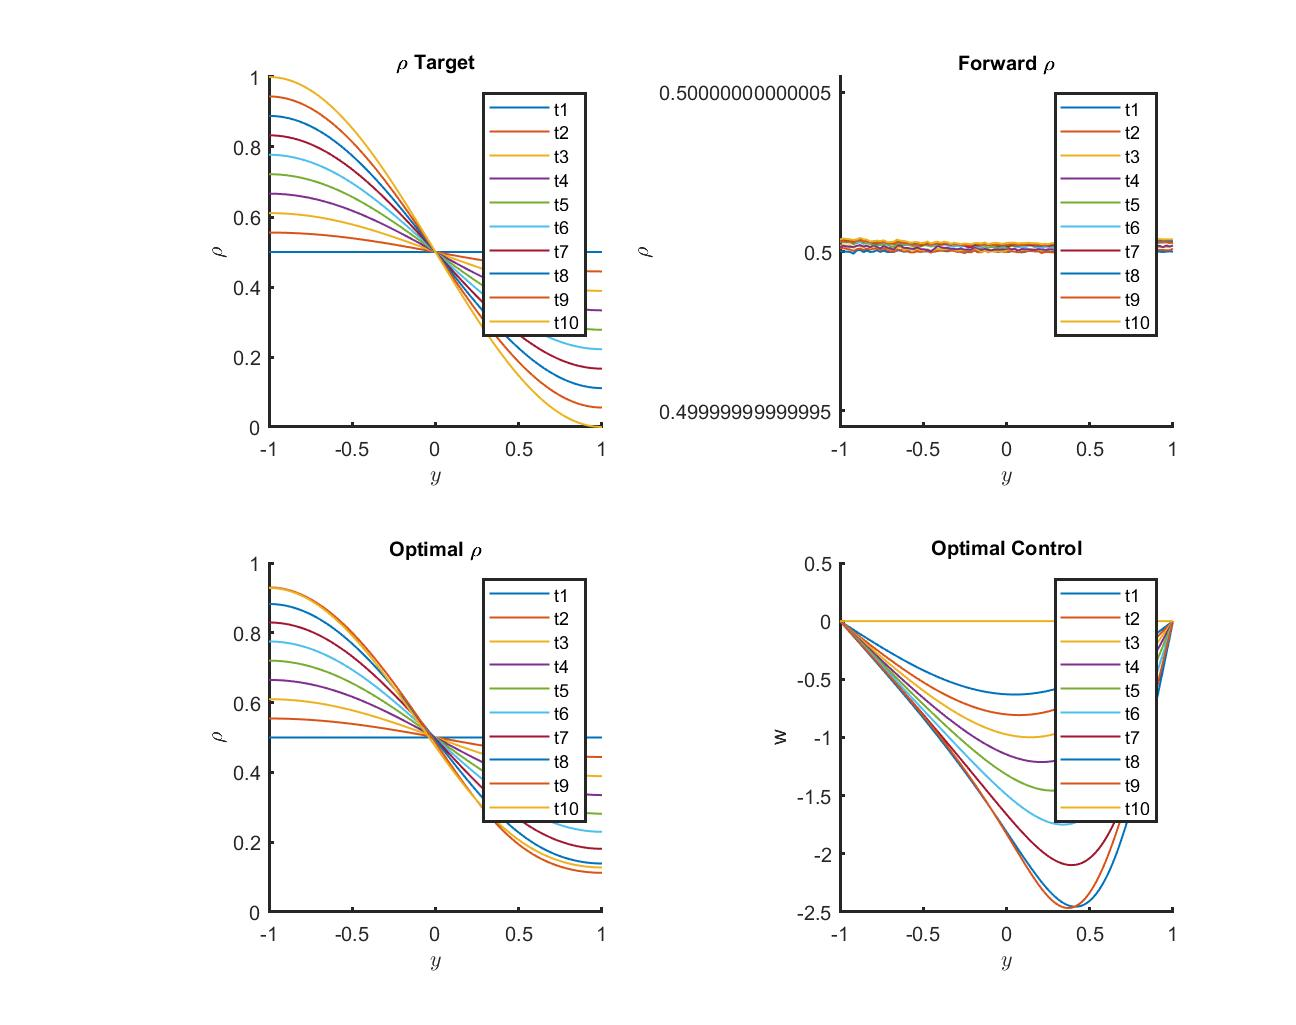
\includegraphics[scale=0.3]{Res03.jpg}
	\caption{Results for Neumann Flow, Asymmetric Example 1, $\gamma = 0$.}
	\label{Res03}
\end{figure}
When $\gamma = -1$, $J_{FW} = 0.0438$ and $J_{Opt} = 0.0011$, see Figure \ref{Resn13}.
\begin{figure}[h]
	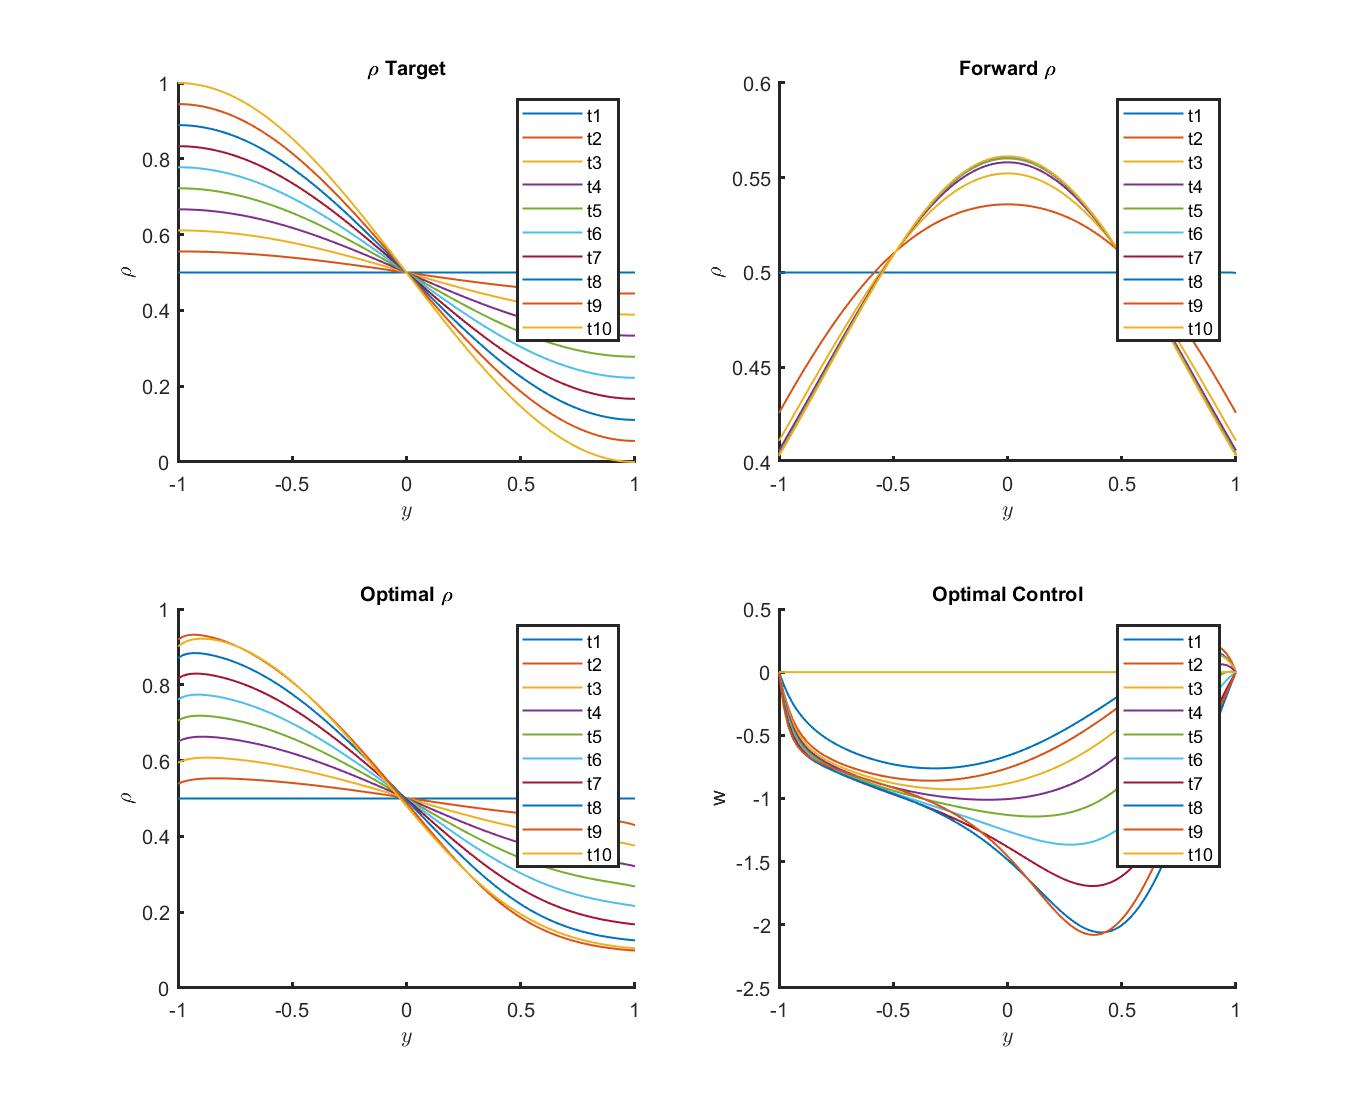
\includegraphics[scale=0.3]{Resn13.jpg}
	\caption{Results for Neumann Flow, Asymmetric Example 1, $\gamma = -1$.}
	\label{Resn13}
\end{figure}
When $\gamma = 1$, $J_{FW} = 0.0434$ and $J_{Opt} = 0.0020$, see Figure \ref{Res13}.
\begin{figure}[h]
	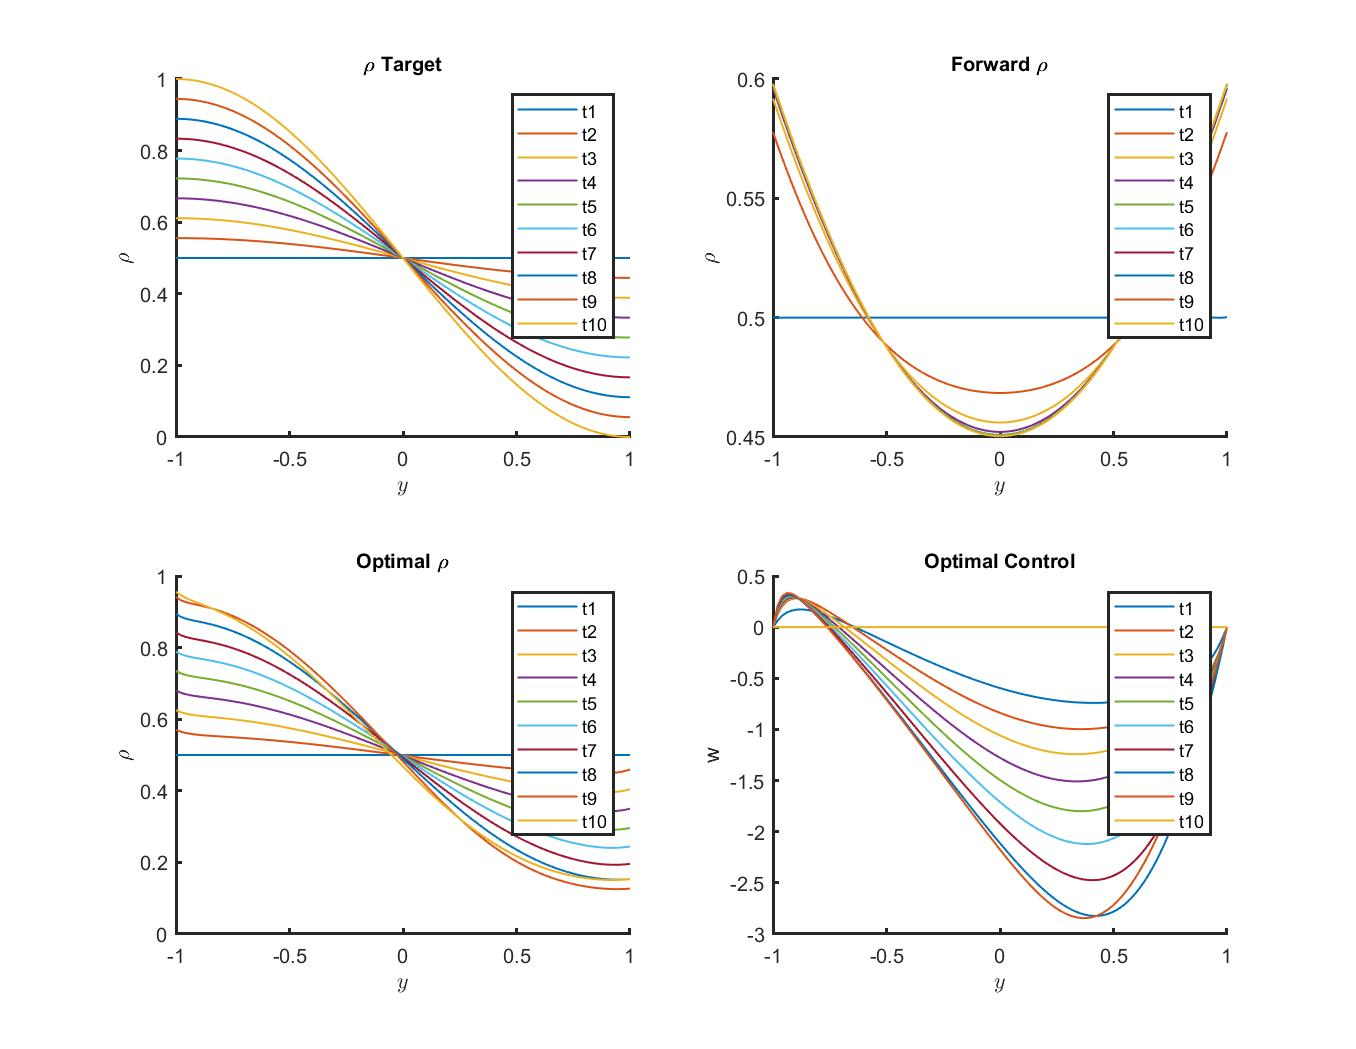
\includegraphics[scale=0.3]{Res13.jpg}
	\caption{Results for Neumann Flow, Asymmetric Example 1, $\gamma = 1$.}
	\label{Res13}
\end{figure}


\section{Neumann Flow Control - Asymmetric Example 2}
For this, the initial condition for $\rho$ is:
\begin{align*}
\rho_{IC} = (-\frac{1}{2}\sin(\pi (y - 2)/2) + \frac{1}{2}),
\end{align*}
and the Flow term is zero in the forward problem.
The target is:
\begin{align*}
\hat \rho = (1-t)(-\frac{1}{2}\sin(\pi (y - 2)/2) + \frac{1}{2}) + t(\frac{1}{2}\sin(\pi(y - 2)/2) + \frac{1}{2}),
\end{align*}
which is similar to the target of the example above but with the new $\rho_{CIC}$ incorporated.

We consider $\beta = 10^{-3}$ and $\gamma = 0$, $\gamma = 1$ and $\gamma = -1$. All of these examples converge in about $700$ iterations and take about $15$ min, using FixPt. $\lambda = 0.01$, $N= 60$, $n = 61$, OLD Tol $= 10^{-8}$, Optimality Tol $=10^{-4}$.
When $\gamma = 0$, $J_{FW} = 0.0321$ and $J_{Opt} = 0.0013$, see Figure \ref{Res04}.
\begin{figure}[h]
	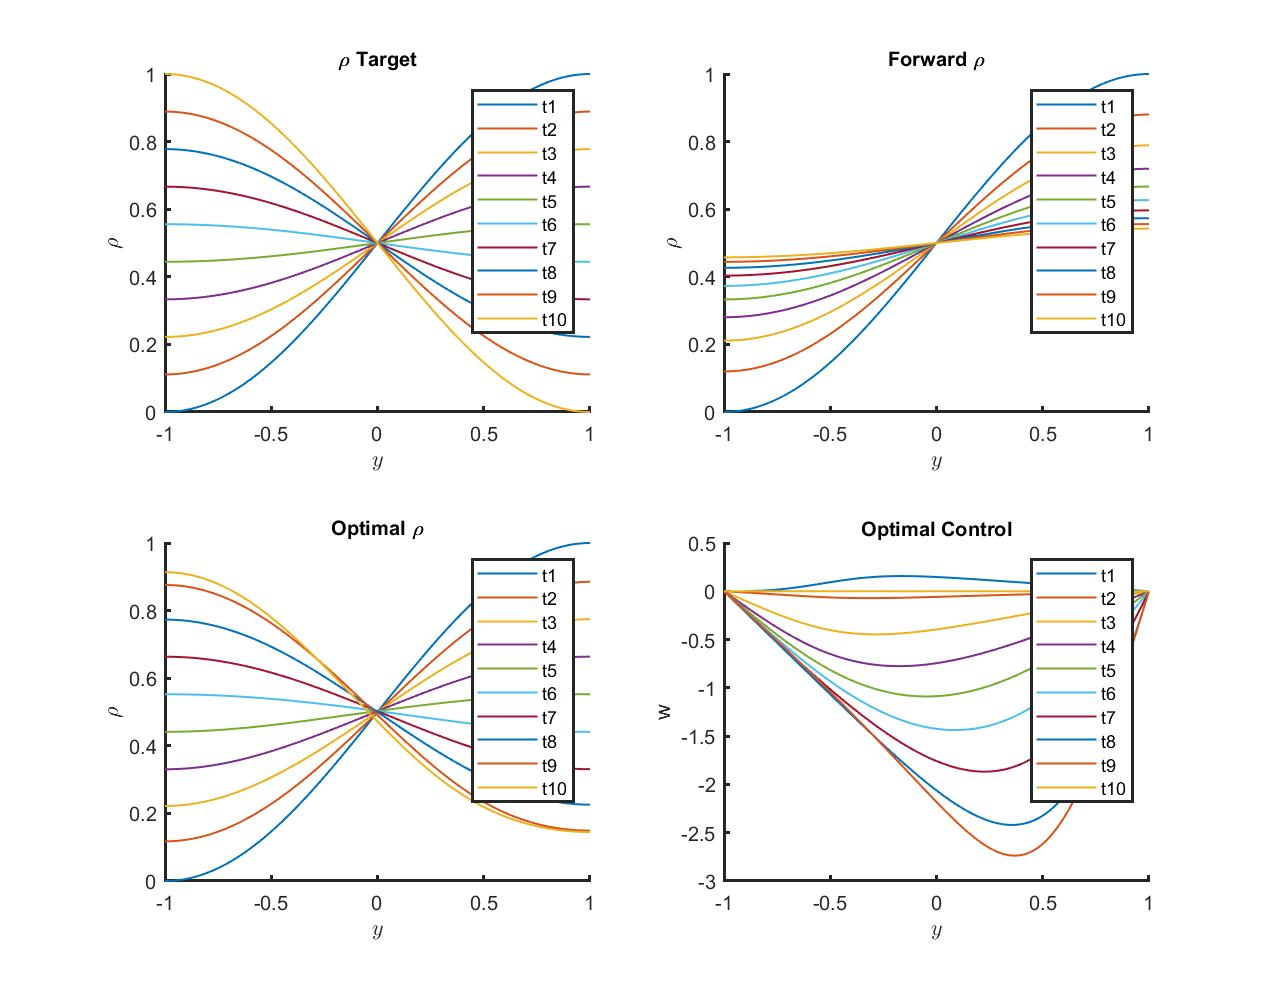
\includegraphics[scale=0.3]{Res04.jpg}
	\caption{Results for Neumann Flow, Asymmetric Example 2, $\gamma = 0$.}
	\label{Res04}
\end{figure}
When $\gamma = -1$, $J_{FW} = 0.0384$ and $J_{Opt} = 0.0012$, see Figure \ref{Resn14}.
\begin{figure}[h]
	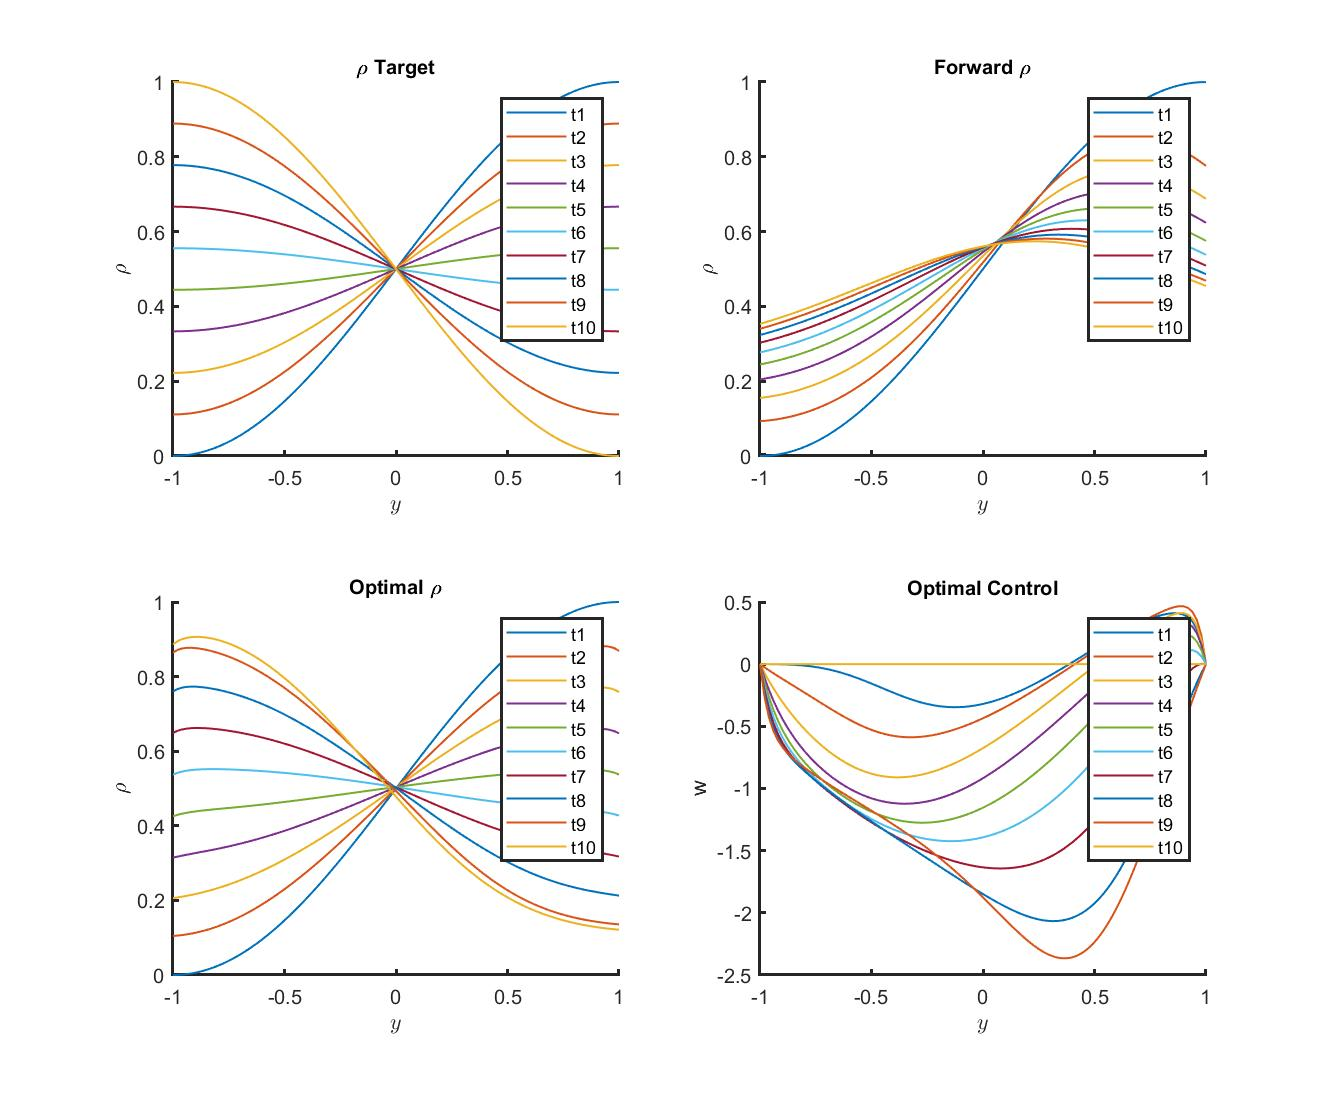
\includegraphics[scale=0.3]{Resn14.jpg}
	\caption{Results for Neumann Flow, Asymmetric Example 2, $\gamma = -1$.}
	\label{Resn14}
\end{figure}
When $\gamma = 1$, $J_{FW} = 0.0307$ and $J_{Opt} = 0.0017$, see Figure \ref{Res14}.
\begin{figure}[h]
	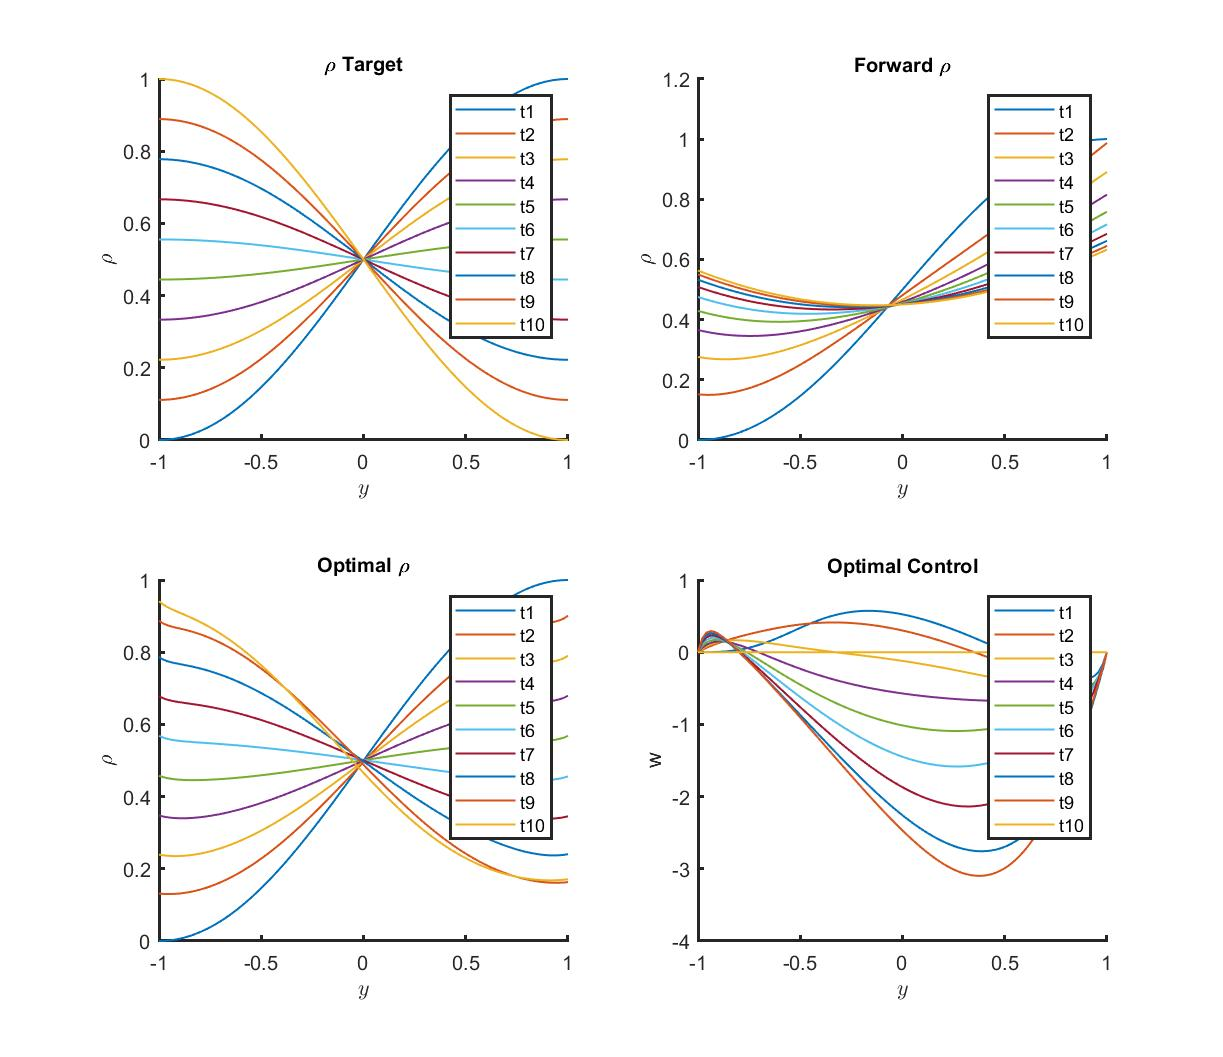
\includegraphics[scale=0.3]{Res14.jpg}
	\caption{Results for Neumann Flow, Asymmetric Example 2, $\gamma = 1$.}
	\label{Res14}
\end{figure}


\section{Dirichlet Flow Control - Symmetric Example}
We take the Dirichlet Boundary condition to be $\rho_{\partial \Omega} = 0.5$. Then the initial condition for $\rho$ is $\rho_{IC}=0.5$, the forward Flow term is zero. 
The target is:
\begin{align*}
\hat \rho = 0.5(1-t) + t(-\frac{1}{4}\cos(\pi y) + \frac{1}{4}).
\end{align*}
We consider $\beta = 10^{-3}$ and $\gamma = 0$, $\gamma = 1$ and $\gamma = -1$. All of these examples converge in under $5$ minutes and about $700$ iterations, using FixPt. $\lambda = 0.01$, $N= 60$, $n = 61$, OLD Tol $= 10^{-8}$, Optimality Tol $=10^{-4}$.
When $\gamma = 0$, $J_{FW} = 0.0313$ and $J_{Opt} = 0.0018$, see Figure \ref{Res02}.
\begin{figure}[h]
	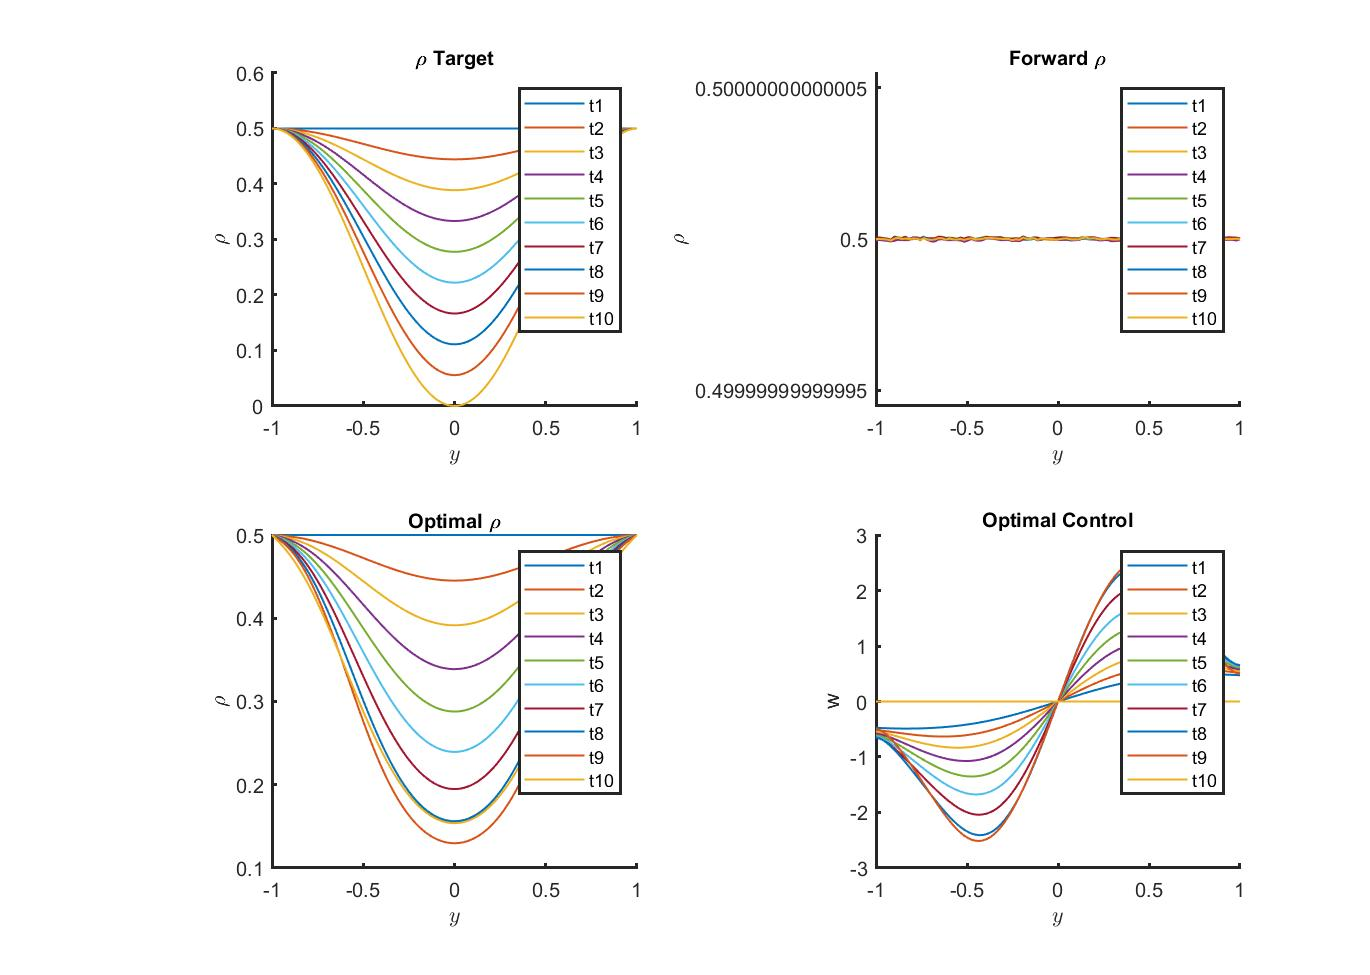
\includegraphics[scale=0.3]{Res02.jpg}
	\caption{Results for Dirichlet Flow, Symmetric Example, $\gamma = 0$.}
	\label{Res02}
\end{figure}
When $\gamma = -1$, $J_{FW} = 0.0741$ and $J_{Opt} = 0.0022$, see Figure \ref{Resn12}.
\begin{figure}[h]
	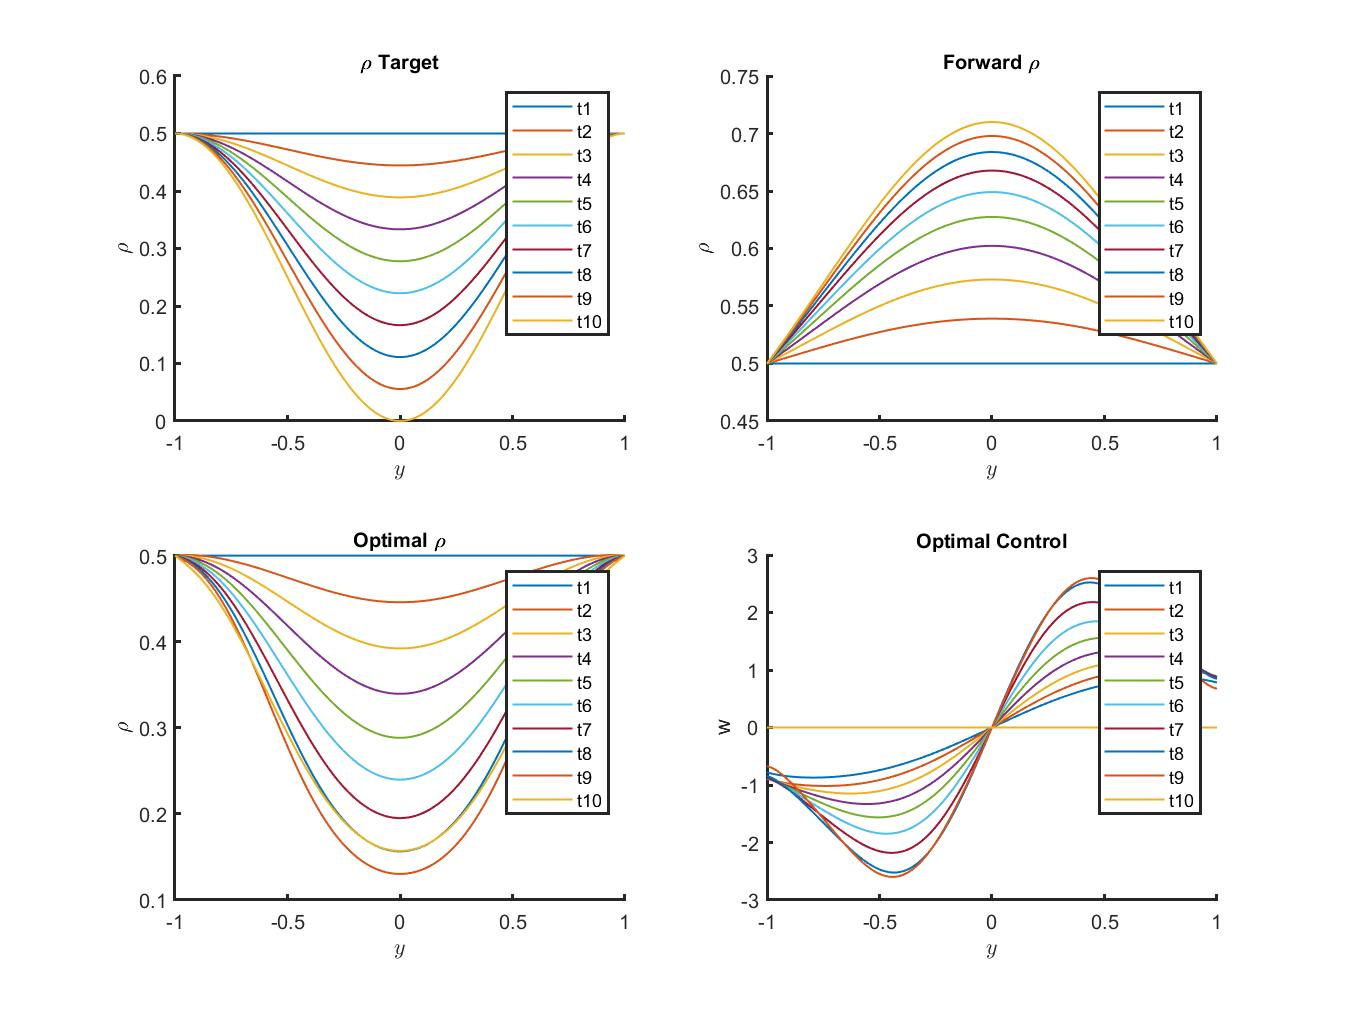
\includegraphics[scale=0.3]{Resn12.jpg}
	\caption{Results for Dirichlet Flow, Symmetric Example, $\gamma = -1$.}
	\label{Resn12}
\end{figure}
When $\gamma = 1$, $J_{FW} = 0.0148$ and $J_{Opt} = 0.0015$, see Figure \ref{Res12}.
\begin{figure}[h]
	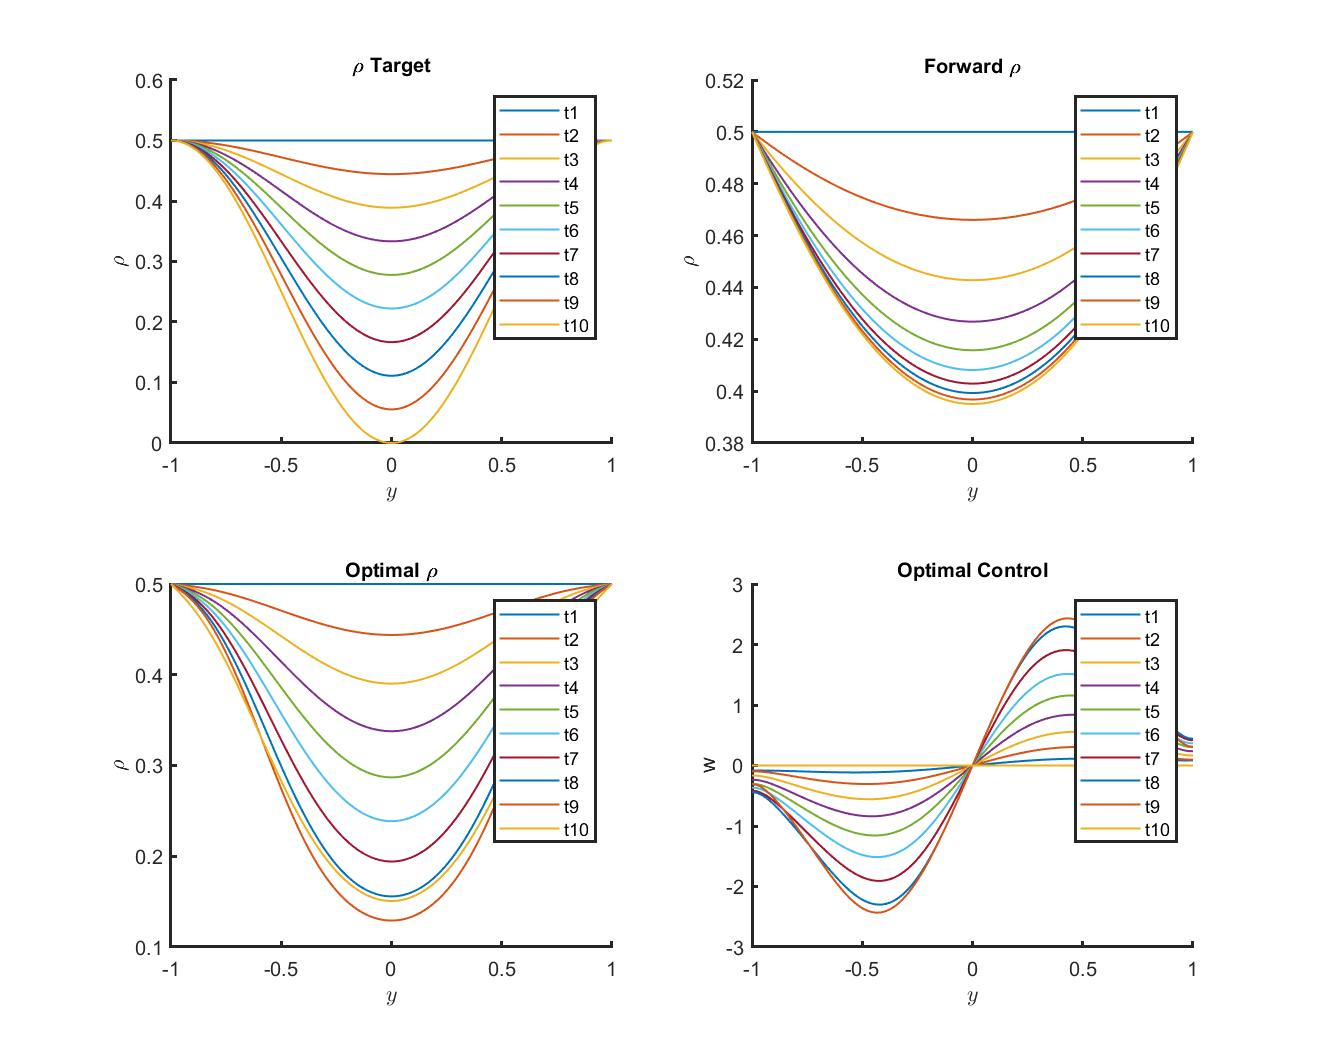
\includegraphics[scale=0.3]{Res12.jpg}
	\caption{Results for Dirichlet Flow, Symmetric Example, $\gamma = 1$.}
	\label{Res12}
\end{figure}
The results for the three cases are slightly but not very visibly different.
\section{Dirichlet Flow Control - Asymmetric Example}

We take the Dirichlet Boundary condition to be $\rho_{\partial \Omega} = 0.5$. Then the initial condition for $\rho$ is $\rho_{IC}=0.5$, the forward Flow term is zero. 
The target is:
\begin{align*}
\hat \rho = 0.5(1-t) + t(\frac{1}{2}(\sin(\pi y) +1)).
\end{align*}
We consider $\beta = 10^{-3}$ and $\gamma = 0$, $\gamma = 1$ and $\gamma = -1$. All of these examples converge in under $5$ minutes and about $700$ iterations, using FixPt. $\lambda = 0.01$, $N= 60$, $n = 61$, OLD Tol $= 10^{-8}$, Optimality Tol $=10^{-4}$.
When $\gamma = 0$, $J_{FW} = 0.0417$ and $J_{Opt} = 0.0027$, see Figure \ref{Res01}.

\begin{figure}[h]
	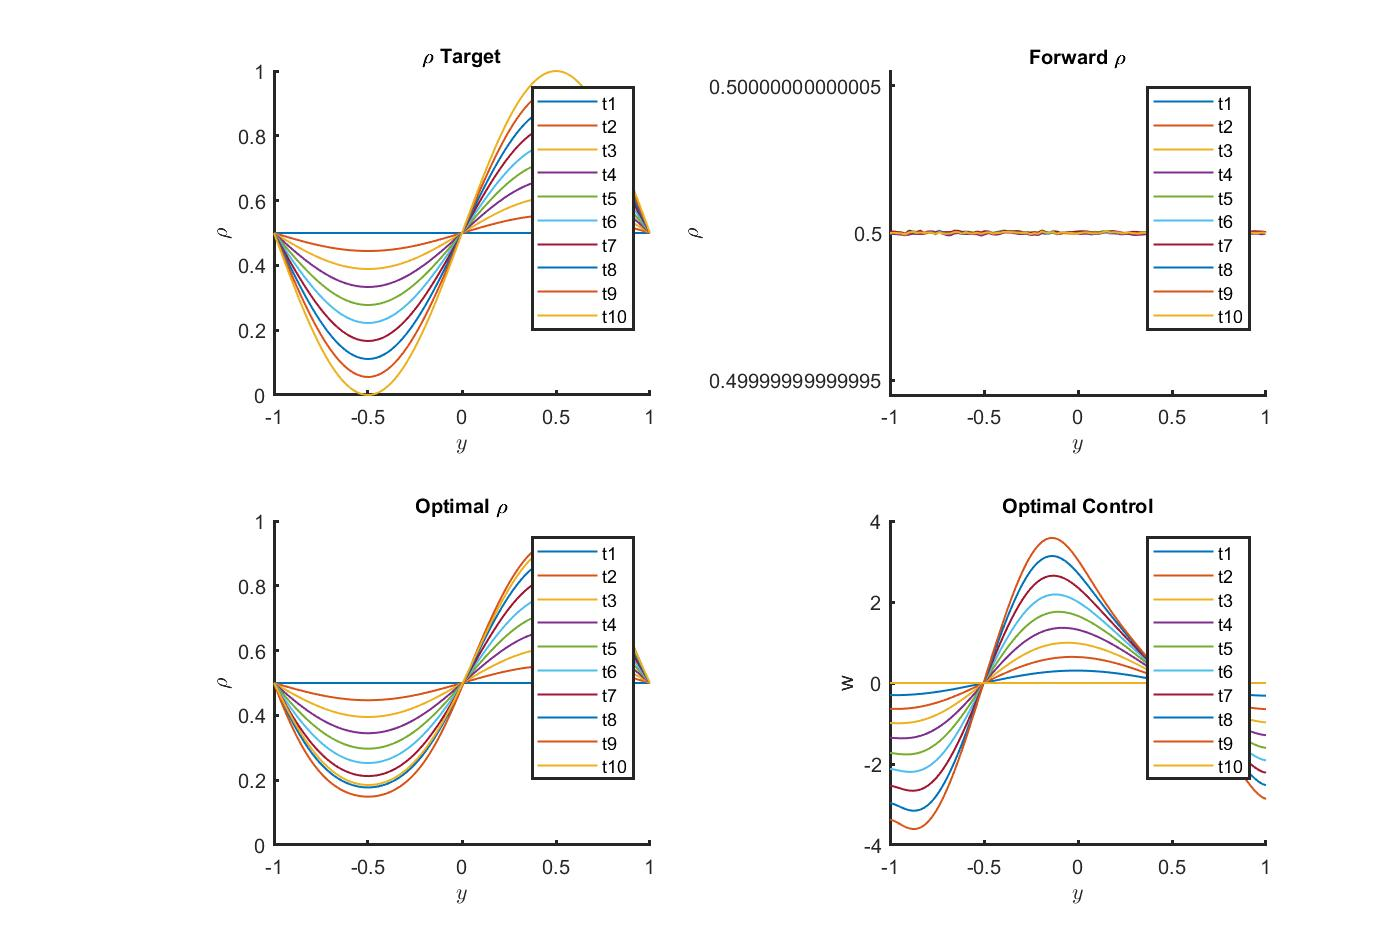
\includegraphics[scale=0.3]{Res01.jpg}
	\caption{Results for Dirichlet Flow, Asymmetric Example, $\gamma = 0$.}
	\label{Res01}
\end{figure}

When $\gamma = -1$, $J_{FW} = 0.0510$ and $J_{Opt} = 0.0026$, see Figure \ref{Resn11}.

\begin{figure}[h]
	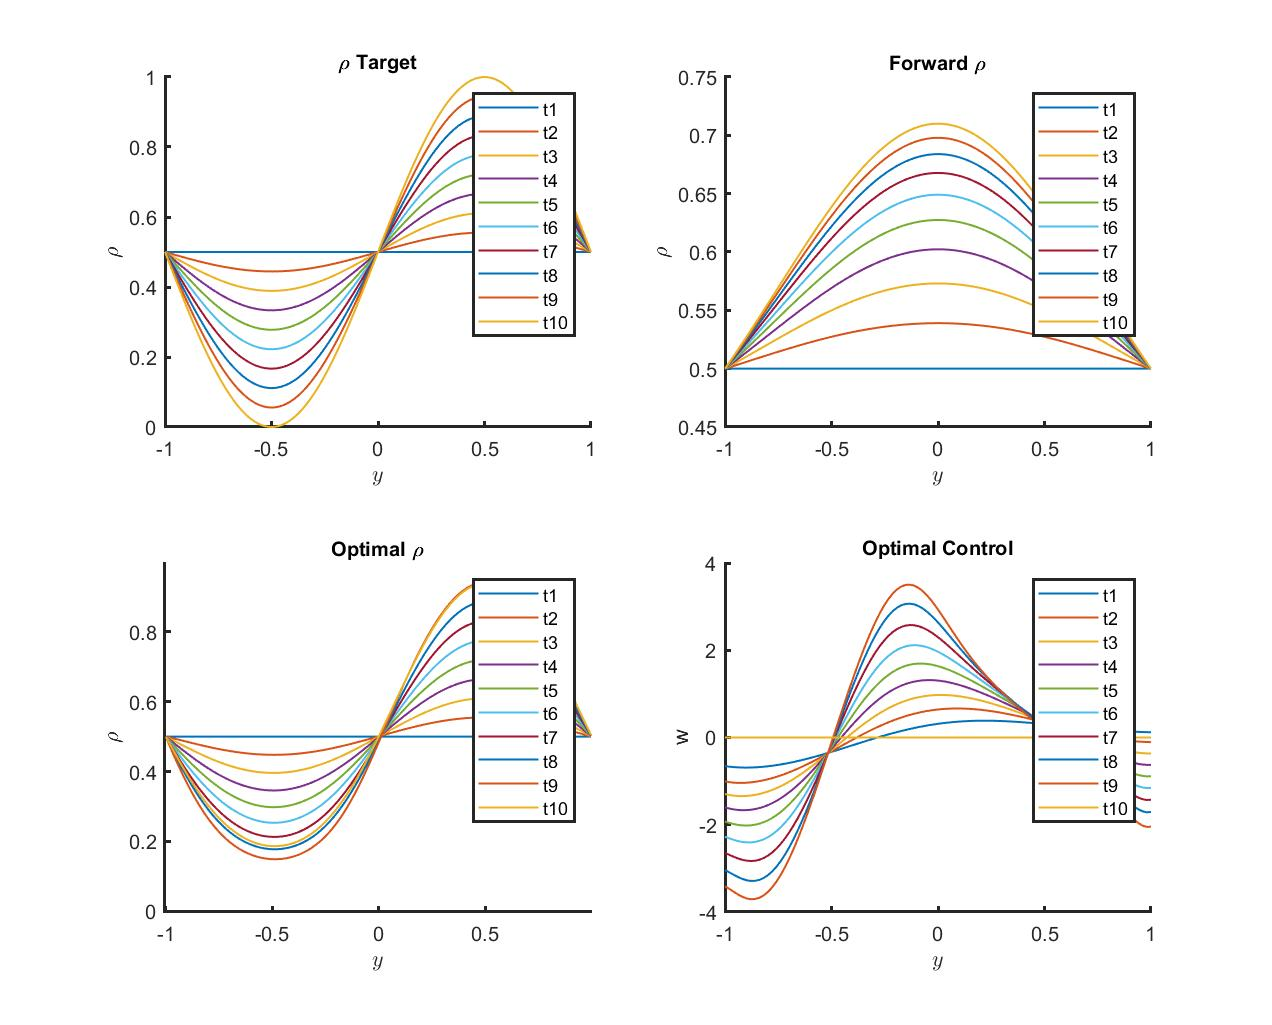
\includegraphics[scale=0.3]{Resn11.jpg}
	\caption{Results for Dirichlet Flow, Asymmetric Example, $\gamma = -1$.}
	\label{Resn11}
\end{figure}

When $\gamma = 1$, $J_{FW} = 0.0452$ and $J_{Opt} = 0.0030$, see Figure \ref{Res11}.

\begin{figure}[h]
	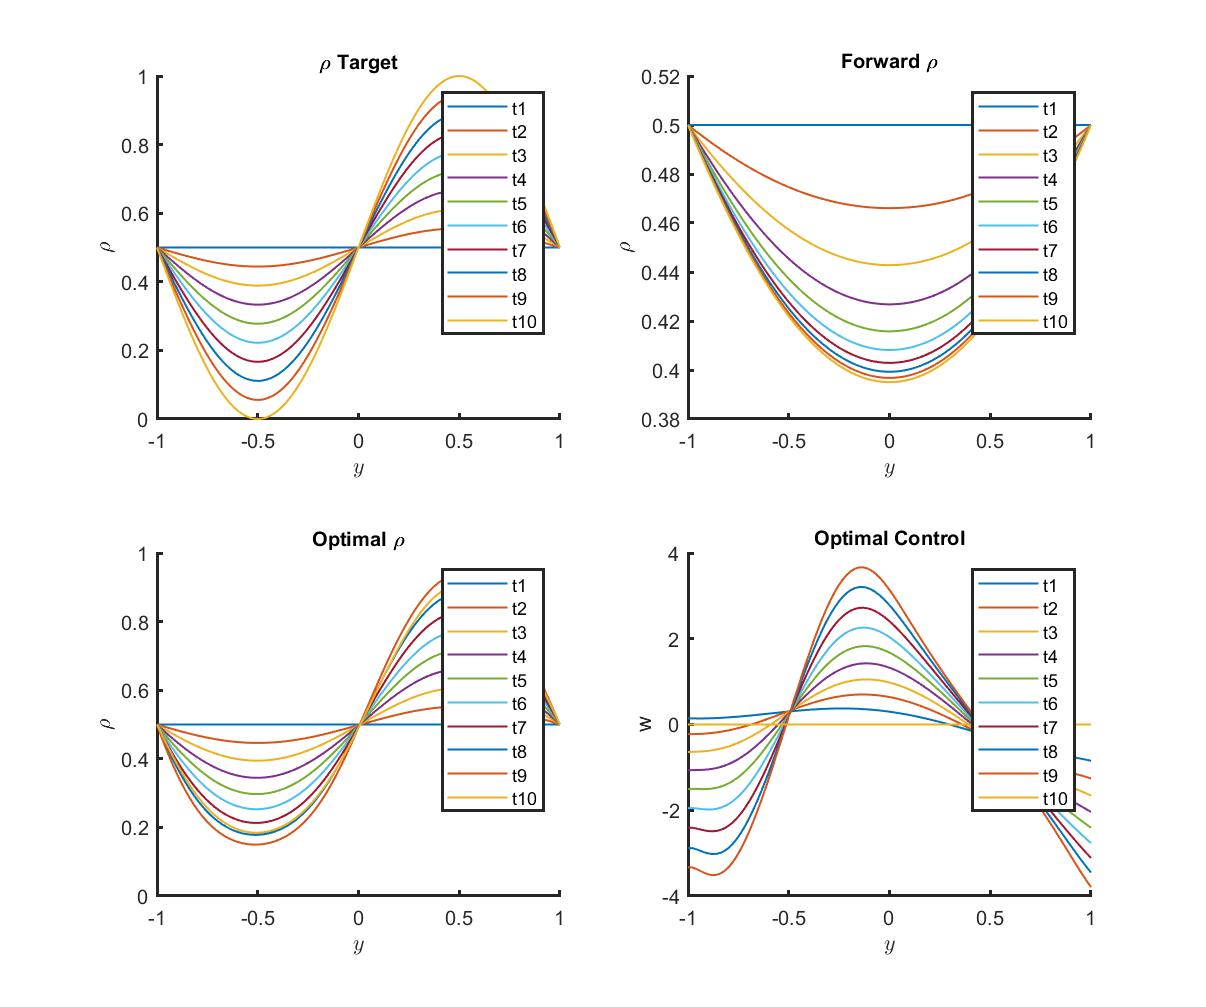
\includegraphics[scale=0.3]{Res11.jpg}
	\caption{Results for Dirichlet Flow, Asymmetric Example, $\gamma = -1$.}
	\label{Res11}
\end{figure}
	
An interesting observation is that even though $J_{FW}$ is smaller for $\gamma =1$, $J_{Opt}$ is smaller for $\gamma = -1$. Overall, the particle interactions don't seem to have a large impact on the results.	
	
	
\end{document}